\BS{[my comment] suggestion for text}

\section{Introduction}
The detection of Gravitational Waves (GW) from compact binary coalescences (CBC) has been possible thanks to the joint effort of a number of different fields of expertise, all joining together to achieve the sophisticated detection process. GW data analysis concerns the detection of a GW signal hidden in the raw detector output (\textit{matched filtering}) and subsequently the inference of its physical properties (\textit{parameter estimation}). In order to accomplish its goal, GW data analysis relies on the availability of waveform (WF) templates to compare with the detector output.
To accurately explore the posterior distribution for the parameters defining a CBC, state-of-the-art parameter estimation (PE) algorithms~\cite{Aasi:2013jjl}~\cite{Veitch2014wba} can require the generation of as many as $10^7$ waveform templates. It is therefore paramount for the waveform generation to be as fast as possible. At the same time, because of the extreme sensitivity to phase differences in the likelihood  function, 
the templates must retain a high degree of accuracy to avoid biases in the posterior exploration.
Many efforts have been devoted to numerically solve Einstein equations for two coalescing objects and 
to predict the gravitational radiation emitted~\cite{}.
As solving the full equations is still extremely computationally challenging, the LIGO-Virgo Collaboration relies on approximate analytical models. 
These can be broadly categorized in  two families; (i) the effective-one-body(EOB) waveform 
models~\cite{Damour:2009kr,Chiaramello:2020ehz}; (ii) the phenomenological 
models~\cite{Khan:2015jqa,Pratten:2020ceb,Estelles:2020osj}.
%
\BS{[would add NRsurrogates]}
%
EOB models are the most complete family 
of analytical models available. They compute the GW signal by solving Hamilton's equations 
and accurately predict the GW signal up to late plunge. The merger and ringdown  parts of 
the signal are then joint to the inspiral signal using information obtained from numerical relativity. 
Because of the numerical integrations involved, they tend to be accurate, but slow to generate, 
see however~\cite{Nagar:2018gnk} for a more efficient approach to obtain the dynamics.

The phenomenological waveforms are based on the post-Newtonian formalism and then calibrated 
to  EOB waveforms and numerical relativity. They tend to be faster than EOB models, but not as accurate.
Many efforts have been devoted to the task of speeding up the generation of GW signals from 
EOB families. For example, one lead to the development of \textit{surrogate models}. Surrogate 
models are constructed starting from some decomposition in the waveform space followed by efficient 
interpolation to avoid any  numerical integration~\cite{Purrer:2015tud,Bohe:2016gbl,Purrer:2017str,Lackey:2018zvw,Cotesta:2020qhw}. 
Being fast to generate, they are routinely employed in GW data analysis. 

A Machine Learning model is a promising alternative to accelerate the
waveforms generation of state-of-the-art models.
Machine Learning (ML) is a branch of statistics that is devoted to reproduce patterns read from data. 
A ML algorithm needs very little human input and, by automatically solving an optimization problem, 
it is able to choose the best performing element among a large  class of parametric models for the solution. 
This is the so-called training procedure. 
The ML flexibility in modeling data and reproducing trends is appealing: with a proper model choice 
and with an appropriate training procedure, we can hope to have a reliable, fast to execute generator 
of GW waveforms, while retaining the accuracy necessary for robust parameter estimation. 
ML procedures have been applied so far to Numerical Relativity 
waveform
data~\cite{Gabbard:2017lja,George:2017pmj,George:2017vlv,Rebei:2018lzh,Khan:2020foe}.
%
\BS{[check
    carefully  refs, I think there are more][also note the Gabbard
    paper uses EOB not NR, I am not sure of the sentence ``ML is
    applied so far to NR'']}
%
The construction of a NR-trained ML waveform model is currently missing except for a very 
restricted region of the parameter space (nonspinning etc.). The main problem behind this is 
because of the absence of a large set of NR simulations ($\simeq 10^{3}$) that would be 
needed to train such an algorithm.

By contrast, an EOB model, informed by NR simulations, does not have such drawback 
since it is designed to generate waveforms all over the BBH parameter space. 
One has indeed to remember that, although NR-informed EOB models are {\it checked} 
only on the part of the parameter space covered by NR simulations, 
they are also typically able to robustly {\it extrapolate} waveforms 
outside this NR-information domain (e.g. large mass ratios and
spins).
%
\BS{[more than extrapolating I would say something technical like] well-defined for any
  adiabatic inspirals from PN knowledge, informed in test-mass regime,
  defined for arbitrary length, etc...}
%
This is, for example, the case of the most  recent avatar of 
the spin-aligned \texttt{TEOBResumS}~\cite{Nagar:2018zoe} model, 
that incorporates subdominant waveform modes,  \texttt{TEOBResumS\_SM}~\cite{Nagar:2019wds,Nagar:2020pcj}. 
This model used several hundreds of the available SXS simulations to inform a highly accurate description 
of the postmerger-ringdown phase~\cite{Damour:2014yha}, but 
only around 40 datasets to improve the behavior of the analytical EOB dynamics, 
suitably modifying the analytical orbital and spin-orbit interaction.
Thus we use \texttt{TEOBResumS\_SM} to train our machine learning 
model for BBH coalescence. For simplicity, we focus here only on the 
dominant $\ell=m=2$ quadrupole waveform. 
We demonstrate that such ML-based model can generate 
GW signals significantly faster than the training model, 
matching the performances of a Reduced Order Modelling 
(ROM)~\cite{Purrer:2015tud,Bohe:2016gbl,Purrer:2017str}.  
At the same time it keeps the same accuracy of the underlying 
training model\footnote{Let us note, in passing, that the ML framework 
is completely general and it works for any EOB model; indeed 
a successful ML model was trained using also the \texttt{SEOBNRv2} 
waveform model~\cite{Taracchini:2013rva}.}.

As a relevant physical application, we use the our ML model \texttt{mlgw} 
to provide a completely new, and independent, analysis of the 10 BBHs 
coalescence events collected in the O1/O2 LIGO-Virgo observing 
runs~\cite{LIGOScientific:2018mvr}. The physical parameters we find are 
compatible with previous analyses obtained with radically different 
models~\cite{LIGOScientific:2018mvr}, though with some
distinguo:
%
\BS{[TEOBResumS or aligned spin effect? this needs to be checked]} 
%
(i) the chirp masses obtained with our model are systematically {\it larger} 
than LVC published results, the mass ratios being systematically {\it smaller}; 
(ii) similarly, the individual spins of the objects, when measurable, are systematically larger than published
results. This is consistent with previously published analysis of GW150914 
data using a slightly different version of \texttt{TEOBResumS}~\cite{Nagar:2018zoe}.

On top of the specific application discussed here, our ML waveform model could also be used directly 
to speed up GW data analysis.
Furthermore, since the time required to generate a WF does not depend
on the signal time length but only only on the number of grid points which the WF is evaluated at,
the applicability of our approach goes far beyond the LIGO/Virgo physics scenario. In particular,
we think about the forthcoming Einstein Telescope, that will be sensitive to very long stellar-mass 
inspirals from 5Hz, or to extreme mass ratio inspiral as LISA sources. In these context the problem
of WF fast generation will be more pressing and our approach, provided a suitable waveform model 
for training,  might be essential for detection and parameter estimation. 

The paper is organized as follows:
in section \ref{sec:setup} we briefly set the notation and the core of the ML problem we solve; in section \ref{sec:model} we describe our model in details; section \ref{sec:performance} we validate the model and assess its accuracy and speed of execution; section \ref{sec:GWTC1} holds our analysis of the GWTC-1 transient catalog; finally in \ref{sec:end} we will report some final remarks and future prospects of our work.

%%%%%%%%%%%%%%%%%%%%%%%%%%%%%%%%%%%%%%%%%%%%%%
%\section{Problem specification}
\section{Conventions setup}
\label{sec:setup}
%--------------------------------------
A binary black hole is parametrized by a vector $ \boldsymbol{\vartheta} = (m_1,m_2, \mathbf{s}_1,\mathbf{s}_2) $, where $m_i$ are the BHs masses and $\mathbf{s}_i = \frac{\mathbf{S}_i}{m_i^2} <1$ are the \textit{dimensionless} spin. 
We call them the \textit{orbital parameters}.
Let the wave direction of propagation be identified with the spherical coordinates $(d_L, \iota, \varphi_0)$, where $d_L$ is the luminosity distance, $\iota$ the polar angle and $\varphi_0$ the azimuthal angle. The polar angle $\iota$ is also called inclination and it is measured with respect to the normal to the orbital plane.
A GW is parametrized as:
\begin{align} \label{eq:h_parametrization}
	&h(t, d_L,\iota,\varphi_0; \boldsymbol{\vartheta}) = h_+ + i h_\times \nonumber \\
		&\qquad= \sum_{l = 2}^{\infty} \sum_{m = -l}^{l} \tensor[^{-2}]{Y}{_{l m}}(\iota, \varphi_0) \cdot H_{lm}(t; \boldsymbol{\vartheta})
\end{align}
where $\tensor[^{-2}]{Y}{_{l m}}(\iota, \varphi_0)$ are the spin-2 spherical harmonics.
We call $(m_1,m_2, \mathbf{s}_1,\mathbf{s}_2, d_L,\iota,\varphi_0)$ \textit{physical parameters} and they fully express the source 
proprieties as well as its orientation and position. In what follows, we will focus on the case in which 
spins $\mathbf{s}_1$ and $\mathbf{s}_2$ are \textit{aligned} with the orbital angular momentum. 
\par
In this work, we concentrate on the single complex quantity $H_{22}$.
Since the dependence on the two angles and distance are known, we fix their value to ${\iota, \varphi_0 = 0}$ and ${d_L = \SI{1}{Mpc}}$ and we only work with waveforms $h_{FIT}(t; \boldsymbol{\vartheta}) = h(t; d_L = \SI{1}{Mpc}, \iota = 0, \varphi_0 = 0, \boldsymbol{\vartheta}) $:
\begin{equation}  \label{eq:h_std}
	h_{FIT}(t; \boldsymbol{\vartheta}) &\equiv \tensor[^{-2}]{Y}{_{2 2}}(0,0) \cdot H_{22}(t; \boldsymbol{\vartheta}) = 4\cdot\sqrt{\frac{5}{64\pi}}H_{22}(t; \boldsymbol{\vartheta}) \; .
\end{equation}
Finally, we express  $h_{FIT}$ in terms of its amplitude and phase
\footnote{Note we adopt a nonstandard sign convention for the phase}:
\begin{equation} \label{eq:h_ML}
	h_{FIT}(t; \boldsymbol{\vartheta}) = A(t; \boldsymbol{\vartheta}) e^{i \phi(t; \boldsymbol{\vartheta})} \; . 
\end{equation}
%%%
We may also write $f_{\boldsymbol{\vartheta}}(t)$ to denote a function $f(t;\boldsymbol{\vartheta})$ of time with parametric dependence on $\boldsymbol{\vartheta}$.
In what follows, $f$ stands for any of the functions $A_{\tilde{\boldsymbol{\vartheta}}}(t)$ and ${\phi}_{\tilde{\boldsymbol{\vartheta}}}(t)$.
\par
With this definition, the full waveform can be expressed as:
\begin{align} 
	&h(t, d_L,\iota,\varphi_0; \boldsymbol{\vartheta}) =  \nonumber\\
		&= {\frac{\SI{1}{Mpc}}{d_L}} \cdot \Bigg\{ \frac{1+\cos^2\iota}{2} \cdot A_{\boldsymbol{\vartheta}}(t)  \cos[\phi_{\boldsymbol{\vartheta}}(t)+2\varphi_0]  \nonumber \\
		&+ i \cdot \cos\iota \cdot A_{\boldsymbol{\vartheta}}(t) \sin[\phi_{\boldsymbol{\vartheta}}(t)+2\varphi_0] \Bigg\}
\label{eq:h_parametrization_simple}
\end{align}
where we split the real and the imaginary part of $h$ and we used the relation ${\tensor[^{-2}]{Y}{_{2 \pm 2}}(\iota, \varphi_0) = (1 \pm \cos \iota)^2 e^{\pm i 2 \varphi_0}}$.
We choose the convention that $\phi_{\boldsymbol{\vartheta}} = 0$ when the amplitude $A_{\boldsymbol{\vartheta}}$ has a maximum
\footnote{Indeed, a constant translation of $\phi_{\boldsymbol{\vartheta}}$ can be absorbed in the definition of $\varphi_0$ and does not affect the physics.}.
\par
\an{All text above should be simplified!!}

%======================
\section{The model \BS{[How about:] MLGW}}
\label{sec:model}
%======================
%
The goal of the present work is to provide an accurate Machine Learning model which outputs the functions $A(t;\boldsymbol{\vartheta})$ and $\phi(t;\boldsymbol{\vartheta})$ (eq.~\eqref{eq:h_ML}), as generated by the state-of-the-art time domain WF models.
Since BBH waveforms trivially scales with the binary mass $M$, we only need to consider 
the variables $\tilde{\boldsymbol{\vartheta}} = (q, s_1, s_2)$, where $q= m_1/m_2 \geq 1$, to describe the waveform's multipoles.
More formally, we seek a ML model that reliably reproduces the following map:
\begin{align}
	(q, s_1, s_2) &\longmapsto A_{(q, s_1, s_2)}(t) \label{eq:objective_amp}\\
	(q, s_1, s_2) &\longmapsto \phi_{(q, s_1, s_2)}(t) \label{eq:objective_ph}
\end{align}

\par
In the context of ML, our task reduces to performing two regressions\footnote{A regression is a statistical method to infer the relationship between a set of ``independent variables" and a set of ``dependent variable". A model consist in a functional form for such relation, usually with many free parameters to be specified. By looking at the data, one should be able to make a proper choice for their value.} 
from $\tilde{\boldsymbol{\vartheta}}$ to the amplitude and phase of WF. 
In order to be able to perform each regression, several steps are required.

\begin{enumerate}[label=(\Alph*)]
	\item \textit{Setting a time grid}. Each WF must be represented on a discrete time grid, which allows for efficient and reliable reconstruction on an arbitrary, user-given, grid. After this operation, the functions $A(t)$ and $\phi(t)$ are represented as vectors\footnote{
In ML jargon, this procedure is called preprocessing and aims to create a standard representation for all the data available (in our case the WFs).
}.
	\item \textit{Creating a dataset of WFs}. A large number of WFs must be generated on the the chosen time grid for a different number of orbital paramter $(q,s_1,s_2)$. This will be the training set for the ML model.
	\item \textit{Reducing the dimensionality of a WF}. In order
          to make the regression feasible, we build a low dimensional representation of the WF}. This operation must be invertible: once a low dimensional representation is given, one should be able to reconstruct the higher dimensional WF.
	\item \textit{Learning a regression}. We train a model to perform the regression from $(q, s_1, s_2)$ to the low dimensional representation of the WF.
\end{enumerate}
We discuss these points in detail in what follows.

%\begin{figure}[!t]
%	\centering
%	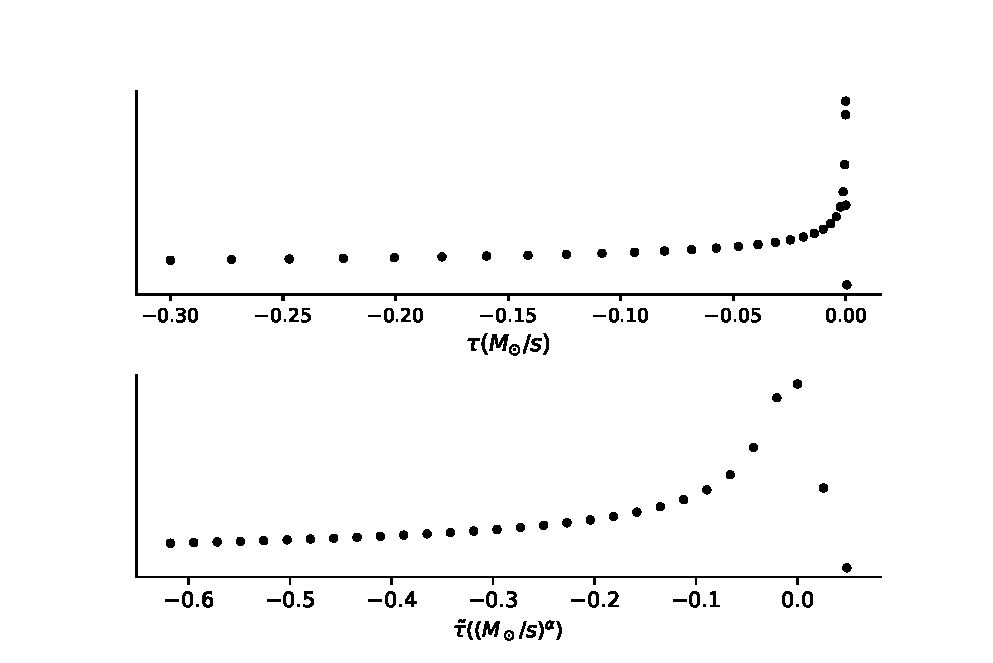
\includegraphics[width=\columnwidth,keepaspectratio]{tau_grid}
%	\caption{Amplitude (arbitrary units) of a GW wave represented on a grid with 30 points.
%It is set $\alpha = 0.3$ and $\tau_{min} = \SI{0.3}{s/M_\odot}$
%The $\boldsymbol{\tau}$ grid is finer around the merger.
%}
%	\label{fig:tau_grid}
%\end{figure}
%
\subsection{The time grid}
Each function $f(t)$ to fit (i.e. amplitude and phase) must be represented by its values $\mathbf{f} \in \R^D$ on a discrete grid of $D$ points $\mathbf{t} \in \R^D$.
It is convenient to work in a grid of (dimensionless) reduced time $\boldsymbol{\tau} = \frac{\mathbf{t}}{M}$.
The time grid is chosen with the convention that at $\tau=0$ the function $A(t;\boldsymbol{\vartheta})$ (i.e. the amplitude of the ${22}$ mode) has a peak.
Once a time grid is set, the vector $\mathbf{f}$ is defined as follows:
\begin{equation}
	\mathbf{f}({\tilde{\boldsymbol{\vartheta}}})_i = f_{{\tilde{\boldsymbol{\vartheta}}}}(\boldsymbol{\tau}_i) \;\;\;\;\;\; i = 1, \ldots D
\end{equation}
\par
The value of $f$ at an arbitrary time must be found by interpolation and this introduces an error in the reconstructed value.
To make the interpolation effective, we introduce a grid adapted to the
  function's variation.
Clearly an equally spaced grid over times is not the best choice since the amplitude has a very narrow peak at $\tau=0$\footnote{As the phase has a rather regular behavior, it is not important to choose the right grid. For this reason a single grid for amplitude and phase, tuned on the behavior of amplitude, is used.}.
A good solution is to build the $\tau$ grid ${\boldsymbol{\tau}}$ as:
\begin{equation} \label{eq:tau_grid}
	{\boldsymbol{\tau}}_i = \sign{\boldsymbol{\tilde{\tau}}_i} \cdot (|\boldsymbol{\tilde{\tau}}_i|)^{\frac{1}{\alpha}} \;\;\;\;\;\; i = 1, \ldots D
\end{equation}
where $\boldsymbol{\tilde{\tau}}_i$ are D equally spaced points in the range of interest and we call $\alpha$ \textit{distortion parameter}.
This choice ensures that more points are accumulated around the peak of amplitude.
\par
The length of the time grid determines the maximum lenght of the WFs that the model can generate.
Let us define $\tau_{min} = -{\boldsymbol{\tau}}_0 > 0 $ the starting point of the grid; thus each WF start at a time $\tau_{min}\cdot M$ before the merger.
Note that $\tau_{min}$ is an important hyperparameter, set by the user, which strongly impacts on the model applicability.
\par
The minimum frequency in the signal as a function of $M, q$ and $\tau_{min}$ is given approximately\footnote{The expression is approximate because it is obtained within a Newtonian framework and does not consider spin effects.
Nevertheless, it gives an useful estimation of the range of the applicability of the model.}
by:
\begin{align}\label{eq:f_min}
	f_{min} = \SI{151}{Hz}  \left( \frac{(1+q)^2}{q} \right)^{\frac{3}{8}}  \left( \frac{M_\odot}{M} \right)  \left(\frac{\SI{1}{ \frac{s}{M_\odot}}}{\tau_{min}} \right)^{\frac{3}{8}}  
\end{align} 


\subsection{Dataset creation}
\label{sec:trainingset}
As in any ML method, we must create a dataset before training any model.
In our case, the dataset consist in a matrix ${X \in \mathbf{Mat}(N,3+2D)}$ of $N$ waveform, which has the following form:
\begin{equation} \label{eq:dataset}
	X_{i:} = [q,s_1,s_2, {A}_{{\tilde{\boldsymbol{\vartheta}}}}^T, \boldsymbol{\phi}_{{\tilde{\boldsymbol{\vartheta}}}}^T]
\end{equation}
where $X_{i:}$ denotes the i-th row of the dataset matrix.
\par
The dataset is filled with random values of parameters ${\tilde{\boldsymbol{\vartheta}}}_i \sim \textrm{Unif}(\mathcal{P})$
\footnote{We denote by $\textrm{Unif}(\mathcal{P})$ a uniform probability distribution on the set $\mathcal{P}$.}.
To generate the training waves the \texttt{TEOBResumS} model is used.
Waves in eq.~\eqref{eq:h_std} are generated with a standard total mass
$M = \SI{20}{M_\odot}$.\BS{[strange sentence (generating waves in an
    equation...) and we just said the total
    mass is not important ... remove?]}
The output of the training model must be interpolated to the chosen time grid.
\par
It is important to ensure that all waves have zero phase at a constant
time point $\bar{t}$: this is crucial to obtain a continuous
dependence of the phase components on the orbital parameters. As model
performances are not seen to depend on the choice of
$\bar{t}$, we arbitrarly set $\bar{t} = 0$.
\par
The range $\mathcal{P}$ of masses and spins covered by the model, as well as the starting point of the grid $\tau_{min}$, can be freely choose by the user, depending on their needs.


%%%%%%%%%%%%%
\subsection{Dimensionality reduction}
Once we are able to represent waveforms, a regressions ${\tilde{\boldsymbol{\vartheta}}} \longmapsto \boldsymbol{A}_{{\tilde{\boldsymbol{\vartheta}}}}, \boldsymbol{\phi}_{{\tilde{\boldsymbol{\vartheta}}}}$ is unfeasible, as the dimension of the target space is too large. Luckily, the elements of $\boldsymbol{A}, \boldsymbol{\phi}$ are strongly correlated with each other: the independent amount of information, required to fully reconstruct the wave, can be stored in a low dimensional vector.
A number of ML techniques to perform such a task are available. Among them, Principal Component Analysis (PCA) \cite[ch. 12]{murphy2012machine} was found to be particularly effective.
\par
The basic idea behind PCA is to seek a \textit{linear relation} between high dimensional and low dimensional data: high dimensional data ($\in \R^D$) are projected onto a $K$ dimensional subspace, by means of an orthogonal projection.
A theorem \cite[sec. 12.2.1]{murphy2012machine} guarantees that, for zero mean data, the generators of subspace are the (orthonormal) first $K$ eigenvectors of the empirical covariance matrix $\Sigma \in \mathbf{Mat}(D,D)$. The eigenvectors are also called Principal Components (PCs) of the data.
Thus, the projection matrix $H\in \mathbf{Mat}(K,D)$ holds in each row the PCs and each high-dimensional point can be effectively expressed as a linear combination of the $K$ PCs\footnote{For this reason, PCA can also be seen as a perturbative expansion of a high dimensional observation. A more realiable reconstruction can be achieved by adding more and more PCs, each of which is less important than its previous.}.
\par
A PCA model is trained with the dataset eq.~\eqref{eq:dataset}: it represents an (approximate) bijective map between the high dimensional WF $\mathbf{f} = \boldsymbol{A}_{\tilde{\boldsymbol{\vartheta}}}, \boldsymbol{\phi}_{\tilde{\boldsymbol{\vartheta}}} \in \R^D$ and the low-dimensional representation $\mathbf{g} = \mathbf{g}_A , \mathbf{g}_\phi \in \R^K$.
%In what follows, $\mathbf{g}$ will be the PCA reduced lower order representation of $\mathbf{f}$ (i.e. of amplitude and phase).
The relation takes the following form:
\begin{align}
	\mathbf{g} = H (\mathbf{f} - \boldsymbol{\mu}) \label{eq:PCA_reduction_model}\\
	\mathbf{f} = H^T \mathbf{g} + \boldsymbol{\mu} \label{eq:PCA_reconstruction_model}
\end{align}
where $\boldsymbol{\mu}$ is the empirical mean vector ${\boldsymbol{\mu} = \frac{1}{N} \sum_{i=1}^N \boldsymbol{f}_i \in \R^D}$ and the matrix $H$ is computed from the empirical covariance ${\Sigma = \frac{1}{N} \sum_{i=1}^N (\mathbf{f}_i-\boldsymbol{\mu}) (\mathbf{f}-\boldsymbol{\mu})^T_i}$.
\par

%%
\subsection{Regression}
Once a dimensional reduction (and reconstruction) scheme is available, we want to perform the regression
\begin{equation} \label{eq:regression_model}
	{\tilde{\boldsymbol{\vartheta}}} \longmapsto \boldsymbol{g}({\tilde{\boldsymbol{\vartheta}}})
\end{equation}
A number of ML models are available for this purpose. The model Mixture of Experts (MoE) \cite{Jacobs1991AdaptiveMoE} \cite[ch. 11]{murphy2012machine} is found to be a good compromise between simplicity and flexibility.
\par
MoE performs the following 1D regression:
\begin{equation} \label{eq:MoE}
	y(\mathbf{x}) = \sum_{l=1}^L (W^T \mathbf{x})_l \cdot \mathcal{S}(V^T\mathbf{x})_l
\end{equation}
where $\mathcal{S}$ is the \textit{softmax function}:
\begin{equation} \label{eq:softmax}
	\mathcal{S}(V^T{\mathbf{x}})_l = \frac{e^{(V^T{\mathbf{x}})_l}}{\sum_{l^\prime = 1}^L e^{(V^T{\mathbf{x}})_{l^\prime}}}
\end{equation}
and ${\mathbf{x}} \in \R^{\tilde{M}}$ and $V,W \in \mathbf{Mat}(\tilde{M},L)$.
The meaning of eq.~\eqref{eq:MoE} is clear: the output is a weighted combination of $L$ linear regressions $(W^T \mathbf{x})_l$ (called \textit{experts}); each expert performs a reliable regression in a small region of the space. The softmax function (in this context also called \textit{gating function}) switches on the expert contributions whenever this is required.
MoE is usually fitted with the Expectation Maximization (EM) algorithm, which iteratively sets the $W$ and $V$ by refining a lower bound to the log-likelihood of the model.
\par
Linear regression is a very simple model, often inadequate to model a complex relation. A simple trick to improve its performance is called \textit{basis functions expansion}. It consist in the replacement:
\begin{equation}
	{\mathbf{x}} \longrightarrow {\boldsymbol{\xi}}({\mathbf{x}}) = [\xi_1({\mathbf{x}}), \ldots, \xi_M({\mathbf{x}})]^T
\end{equation}
Thus, each expert becomes a non linear regression of the input ${\mathbf{x}}$.
A careful choice of basis functions can really make a difference in fit performances and it must be done at validation time, by comparing performances of different models.
\par
The user must choose the number $L$ of experts and the basis functions features ${\boldsymbol{\xi}}({\tilde{\boldsymbol{\vartheta}}}) \in \R^{M}$ to use.
Including in the $\xi_i$ every monomial up to 3/4th order in the three variables $ (\log q, s_1, s_2)$ seems a good working choice for our model
\footnote{
The choice of working with variable $\log q$ rather than $q$ gives much better validation results.
Heuristically, using $\log q$ prevents the values of the data features to vary too much within the range of interest, yielding more stable numerical performance.
}.
\par
%The MoE is fitted with a reduced dimensional version of dataset~\eqref{eq:dataset}:
%\begin{equation} \label{eq:dataset_MoE}
%	G_{i:} = [q,s_1,s_2, \mathbf{g}_{A}(\tilde{\boldsymbol{\vartheta}})^T, \mathbf{g}_{\phi}(\tilde{\boldsymbol{\vartheta}})^T]
%\end{equation}
As MoE model deals with single dimensional outputs, a single independent regression must be performed for each component $g_k$ of $\mathbf{g} \in \R^K$
\footnote{This is not a great limitation, because, due to orthogonality of PCs, each $g_j$ is independent from the other: we do not miss correlation among different regressions.}.
In general, a regression will be a collection of MoE weights ${\{ W^{(k)}, V^{(k)} \in \mathbf{Mat}(M,L_k) \}_{k=0}^K}$, where index $k$ labels different regressions for each PC.

\subsection{Summary}
The model has the following explicit form:
\begin{align}
	& \textrm{model}: \mathcal{P} \subset \R^3 \rightarrow \R^K \rightarrow \R^D \nonumber\\
	& {\tilde{\boldsymbol{\vartheta}}}
	\longmapsto  \mathbf{g}({\tilde{\boldsymbol{\vartheta}}} ) = 
		\begin{pmatrix}
		\sum_{l=1}^{L_1} (W^{(1)\;T} \boldsymbol{\xi})_l \cdot \mathcal{S}(V^{(1)\;T}\boldsymbol{\xi})_l \\
		\vdots \\
		\sum_{l=1}^{L_K}  (W^{(K)\;T} \boldsymbol{\xi})_l \cdot \mathcal{S}(V^{(K)\;T}\boldsymbol{\xi})_l
		\end{pmatrix}
	\nonumber \\	
	& \qquad \qquad \qquad \longmapsto \mathbf{f}({\tilde{\boldsymbol{\vartheta}}} ) = H^T \mathbf{g}({\tilde{\boldsymbol{\vartheta}}} ) + \boldsymbol{\mu} \label{eq:model}
\end{align}
where ${\boldsymbol{\xi}}({\tilde{\boldsymbol{\vartheta}}}) \in \R^M $ are the chosen basis function for the regression and $\mathcal{S}(\cdot)_k$ is the \textit{softmax} function eq~\eqref{eq:softmax}.
Two relations of the same type must be fitted, one for the amplitude, the other for the phase.
\par
Once weights are set properly, the expression provides an estimation for the waveform $h_{FIT}$ in \eqref{eq:h_std}.
The fitted expression for  $h_{FIT}$ is evaluated at constant mass $M = \SI{20}{M_\odot}$; the dependence on total mass is inserted analytically and the dependence on $(d_L, \iota, \varphi_0)$ is computed with eq.~\eqref{eq:h_parametrization_simple}.
We are thus able to obtain a complex waveform $h(t;m_1,m_2, s_1, s_2, d_L, \iota, \varphi_0)$ which reproduces closely a waveform from the training model.
The model can extrapolate outside the range of train orbital parameters, without guarantee of reliable results.
\par
Note that equation \ref{eq:model} can be used to compute a closed form expression for the gradients of the waveform with respect to the orbital parameters. Such calculations are included in the released version of \texttt{mlgw}.

%%%%%%%%%%%%%%%%%%
\section{Model performance}
\label{sec:performance}
We now discuss some tests on our model. We first study how its performance depends on the choice of hyperparameters. Furthermore, we assess the model accuracy and its limitations.
Finally, we measure the speed up provided by our model as compared with training \texttt{TEOBResumS} model.
As it is common, we measure the similarity between two waves by means of the \textit{optimal mismatch}:
\begin{align}
	\bar{\mathcal{F}}[h_1,h_2] &\equiv 1- \frac{\langle h_1, h_2 \rangle}{\sqrt{\langle h_1, h_1 \rangle \langle h_2, h_2 \rangle}}	\label{eq:mismatch_def}
\end{align}
where, as usual, we defined the \textit{Wiener product} as:
\begin{equation}
	 {\langle h_1, h_2 \rangle} = 4 \int_0^\infty \d{f} \; \frac{h_1^*(f) h_2(f)}{S_n(f)}
	\label{ew:Wiener}
\end{equation}
In the equation above, $S_n(f)$ is the detector's noise curve and the $*$ denotes complex conjugate.
In what follows, we always use a flat noise curve (i.e. constant power spectral density for the detector noise).
%%%%%%%

\subsection{Validation}
Wherever relevant, we will employ a dataset with $5800$ waveforms generated in the domain $\mathcal{P} = [1,20]\times[-0.8,0.95]\times[-0.8,0.95]$, with $\tau_{min} = \SI{1.0}{s/M_\odot}$. The dataset was generated with TEOBResumS model \cite{}.
\paragraph{Dataset generation parameters}
We first evaluate the impact of number of grid points $N_{grid}$ and distortion parameter $\alpha$.
Let $\mathbf{f}_{N_{grid}, \alpha}$ the wave stored in a dataset where $\tau_{min}$ and $\mathcal{P}$ are fixed as above. We compare it with the output of the EOB model $\mathbf{f}_{EOB}$.
We then vary $N_{grid}$ and $\alpha$ and report the resulting mismatch $\mathcal{F}[\mathbf{f}_{EOB}, \mathbf{f}_{N_{grid}, \alpha}]$ in figure \ref{fig:N_grid}.
%%
\begin{figure}[!t]
	\centering
	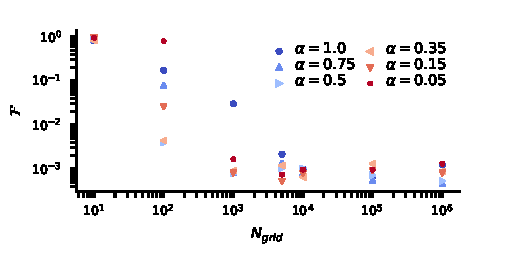
\includegraphics[width=\linewidth,keepaspectratio]{N_grid}
	\caption{Mismatch between waves $\mathbf{f}_{N_{grid}, \alpha}$ and raw waves from EOB model, as a function of time grid size $N_{grid}$. Each series refers to a different values of $\alpha$.
Mismatch is computed on $10$ test waves.  textwidth: \printinunitsof{in}\prntlen{\linewidth}
%The raw wave from EOB is evaluated at the original time grid provided by EOB: this means that it spans $\sim \SI{4}{s}$ sampled at $10^5$ step per second.
}
	\label{fig:N_grid}
\end{figure}
\par
As expected, we note that, by increasing the number of grid points, the mismatch decreases. Furthermore, using more than $\sim 10^3$ grid points, does not bring any improvement to mismatch. In this case, the result is dominated by numerical errors in the interpolations and it provides a lower-bound for the performances of the fit.
A careful choice of $\alpha$ provides a remarkable improvement when $N_{grid}$ is small. For a high number of grid points, different values of $\alpha$ yield almost equivalent results.
A good setting for dataset hyperparameters might be: $N_{grid} \simeq 2/3 \cdot 10^{3}$ and $\alpha \simeq 0.3/0.5$.
%%%%
\begin{figure}[!t]
	\centering
    \begin{minipage}{.5\linewidth}
        \centering
        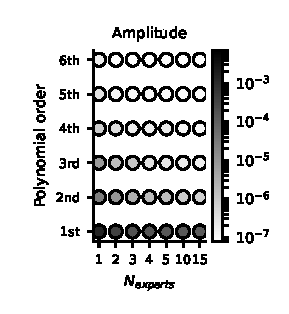
\includegraphics[width=\linewidth]{MoE_mismatch_amp}
    \end{minipage}\hfill
    \begin{minipage}{.5\linewidth}
        \centering
        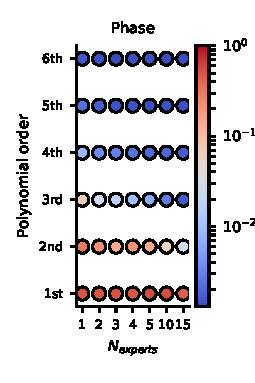
\includegraphics[width=\linewidth]{MoE_mismatch_ph}
    \end{minipage}
	\caption{Validation results for fit of MoE model. Each point corresponds to a MoE regressions for the amplitude (left) and phase (right), with a different values of expert number $N_{exp}$ and order of polynomial basis function.
The amplitude and phase are represented with 5 and 4 PCs respectively.
In the colorbar, we represent the mismatch on test waves: it is obtained by reconstructing test waves with fitted amplitude (phase) and test phase (amplitude).
}
	\label{fig:MoE_test}
\end{figure}


\paragraph{MoE parameters}
We only focus on setting the number of experts $N_{exp}$ for each component model and the basis functions $\xi_i(\boldsymbol{\tilde{\vartheta}})$ to use in the regression. Other parameters, related to the details of the training procedure, will not be considered here.
\par
In figure \ref{fig:MoE_test} we present our results.
We fitted a model for amplitude (or phase) for different configurations of expert number $N_{exp}$ and polynomial basis function.
By label ``n-th order", we mean that in the basis function expansion, every monomial up to n-th order is used.
We report with a colorbar the value of the mismatch $F$ between test and reconstructed WFs. The MoE models for each component share the same number of experts $N_{exp}$.
The test mismatch for the fitted amplitude (phase) is computed by using the test phase (amplitude) in the reconstructed wave.
\par
As a general trend, fit performance improves whenever the model complexity (i.e. number of fittable parameters) increases.
In general, we note that adding more features is more effective than employing the number of experts.
However, the model performance does not improve indefinitely: as we see in figure \ref{fig:MoE_test}, many ``complex" models show similar performance, regardless their complexity.
A model with 4 experts and 4th order polynomial regression is the ``simpler" of such models and thus it should be deemed as the best choice.
%%%%%%%%%
\begin{figure}[!t]
	\centering 
    \begin{minipage}{.5\linewidth}
		\centering
	    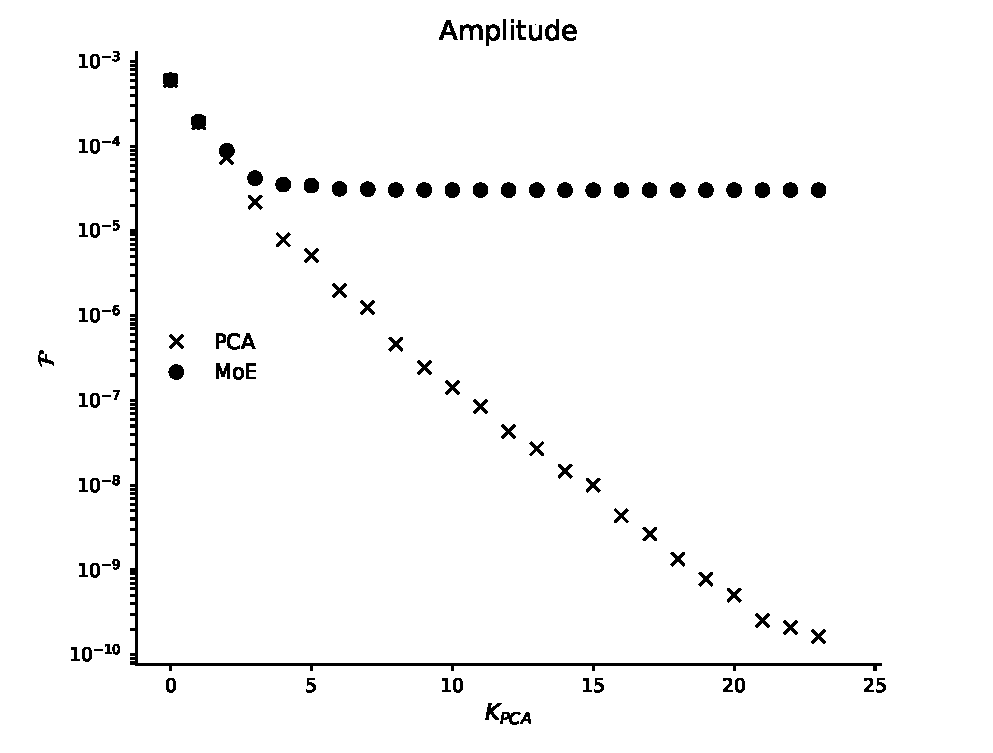
\includegraphics[width=\linewidth]{mismatch_MoE_vs_PCA_amp}
	\end{minipage}\hfill
    \begin{minipage}{.5\linewidth}
		\centering
	    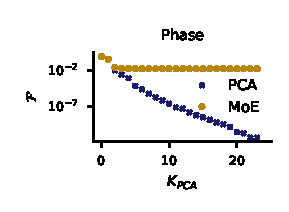
\includegraphics[width=\linewidth]{mismatch_MoE_vs_PCA_ph}
	\end{minipage}
	\caption{Test mismatch as a function of the number of PCs used in the low dimensional representation.
Label "PCA" refers to waves reconstructed with PCA only; points with label "MoE" are reconstructed after a MoE regression.
Data refers to amplitude (left panel) and phase (right panel).
MoE model is chosen to be the optimal one with $4$ experts and a fourth order polynomial.
}
	\label{fig:mismatch_MoE_vs_PCA}
\end{figure}
%%%%%%%%%
\paragraph{Choosing the number of PCs}
Of course, the accuracy of the reconstruction of the low dimensional representation depends on the number $K$ of principal components considered: the more PCs are used, the best accuracy can be achieved.
However in practice, due to error in the MoE regression, one cannot reduce the reconstruction mismatch
arbitrarily\footnote{Indeed, at high PC order the relations to fit become noisy and the regression becomes less accurate, eventually washing out any improvement brought by a higher number of PCs.}
and one should choose the number of PCs, while checking MoE performance.
\par
In figure \ref{fig:mismatch_MoE_vs_PCA} we report a numerical study of this. We plot the reconstruction mismatch as a function of the number of PCs considered. We consider separetely the amplitude and the phase. In one series, we reconstruct the wave using true values of PCs: the mismatch is a measure of PCA accuracy. In the other, we reconstruct a wave using values for PCs as guessed by MoE regression: this is a measure of accuracy of both PCA and regression.
For the first two PCs, the regression is accurate enough for reproducing the PCA accuracy.
On the other hand, any regression beyond the 4th PCA component does not give any improvement to the MoE mismatch: the noise in the relation of high order PCs is too high for a regression to be performed.
\par
In the PCA, we include every PC which yields improvement in MoE mismatch. For our model, $K = 5(4)$ is a good choice for amplitude (phase).
Of course, this strongly depends on the regression model: the more precise the model is, the more PCs can be included.
However, any model cannot increase its accuracy indefinitely. Every training model has an intrinsic noise level, due to numerical error and to the approximations in the physical model.
%%%%%%%%%%%%%
\paragraph{Choosing the number of training points}
The choice of the number of training points $N_{train}$ must trade between accuracy and speed of execution. Too many training points will make the training slow, while too few training points will yield a poor model, which does not generalize the data (underfitting).
In the choice of number of training points, the comparison between train and test error will provide important information on how the model is able to generalize the trend.
\par
In figure \ref{fig:N_train} we report train and test value of mismatch and mse of first 3 PCs as a function of the number of training points. Data refers to a MoE model fitted for 4 PCs of the phase dataset. The models has ${N_{exp} = 4}$ and performs basis function expansion with a 4th degree polynomial.
\begin{figure}
	\centering
    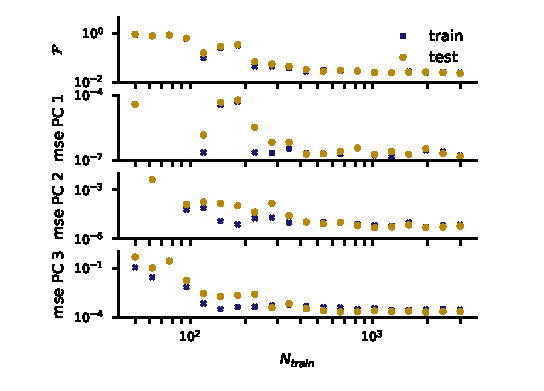
\includegraphics[width=\linewidth]{N_train}
	\caption{Train and test error for MoE fit of 4 PCs of phase, as a function of the number of training points. We report train and test reconstruction mismatch (top) and mse for the first 3 PCs (below).
    MoE model employs 4 experts and a fourth order polynomial for a basis function expansion.
	Test mismatch are obtained using test amplitude to reconstruct the waveform; this is not a great limitation as any error in phase reconstruction dominates the overall mismatch.
    }
	\label{fig:N_train}
\end{figure}
\par
As $N_{train}$ increases, we see a steady decrease of the errors, until a plateau is reached.
Since for a reasonably high number of training points ($N_{train} \gtrapprox 50$) train and test error are close to each other, we note that overfitting is not a problem.
For $N_{train} \gtrapprox 800$, the trend stabilises and increasing training points does not affect much model performance.
In the present model, setting $N_{train} \simeq \SI{3000}{}$ is a good choice
\footnote{As compared with standard neural networks, which routinely employ $O(10^5)$ points datasets, this is an incredibly low amount of data. This is due to the fact that MoE is a simple model with a few number of parameters: few data are enough for learning a reliable relation.}.
%%%%%%%%%%%%%%%%%%%%%%
\subsection{Accuracy}
%%%%
\begin{figure}
	\centering
    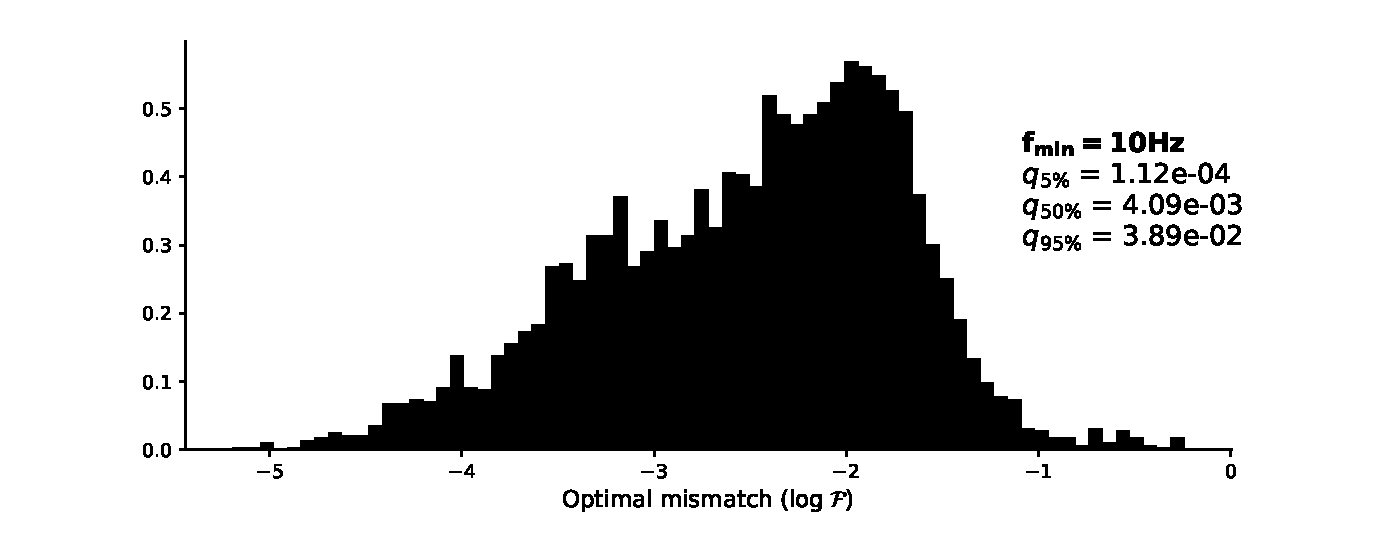
\includegraphics[width=\linewidth]{F_hist}
	\caption{Histogram for the logarithm of mismatch values, computed on $N=4000$ test waveforms. Each WF is generated with random orbital parameters $(m_1,m_2, s_1, s_2, d_L, \iota, \phi_0)$ and with a starting frequency of $\SI{10}{Hz}$.
We report the median value $q_{50\%}$ as well as the positions $q_{5\%}$ and $q_{95\%}$ of the 5th and 95th percentile.
The $95\%$ of the test waves have a mismatch lower than $7.5 \cdot 10^{-3}$.
}
	\label{fig:F_hist}
\end{figure}
%%%%
We compute mismatch value on a number of WFs with random values of the physical parameters (i.e. $m_1,m_2, s_1, s_2, d_L, \iota, \varphi_0$) for each wave.
We report our results in the histogram in figure~\ref{fig:F_hist}.
We report a median value of the distribution $\mathcal{F}_m = 5.5 \cdot {10^{-4}}$. Such results are similar to the discrepancies between state-of-the-art models.\BS{REFS}
\par
To understand better model performances, it is interesting to display the accuracy as a function of the orbital parameters $\boldsymbol{\vartheta} = (q,M,s_1,s_2)$.
We generate waves for randomly chosen values of $\vartheta = (q, M, s_1, s_2)$ and, for each wave, we measure test mismatch $\mathcal{F}$ and mse on the reconstruction of the first PC for the phase.
The latter is useful to test the accuracy of the fit before wave reconstruction.
The results are reported in the contour plots in figure \ref{fig:countour}.
\sschmidt{Probably the comments below are not really interesting...}
\par

%%
\afterpage{
\begin{figure}[!ht]
	\newcommand{\minipagesize}{.5}
	\newcommand{\titlefontsize}{7}
	\centering 
    \begin{minipage}{\linewidth}
        \centering
	 	\begin{minipage}{\minipagesize\linewidth}
		    \centering
			{\fontfamily{DejaVuSans-TLF} \fontsize{\titlefontsize}{12}\selectfont 
			Mismatch%
			} \\
			\vskip0.3em
		    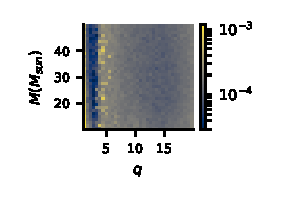
\includegraphics[width=\linewidth]{F_countour_mass}
		\end{minipage}\hfill
		\begin{minipage}{\minipagesize\linewidth}
		    \centering
			{\fontfamily{DejaVuSans-TLF} \fontsize{\titlefontsize}{12}\selectfont 
			Mean Squared Error%
			} \\
			\vskip0.3em
		    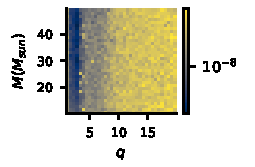
\includegraphics[width=\linewidth]{mse_countour_mass}
		\end{minipage}
    \end{minipage}\hfill
    \begin{minipage}{\linewidth}
        \centering
	 	\begin{minipage}{\minipagesize\linewidth}
		    \centering
		    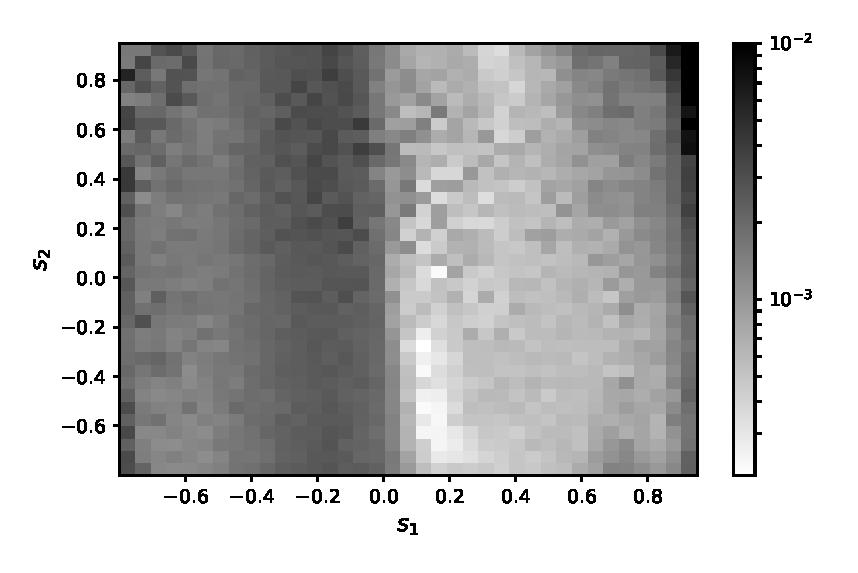
\includegraphics[width=\linewidth]{F_countour_spins}
		\end{minipage}\hfill
		\begin{minipage}{\minipagesize\linewidth}
		    \centering
		    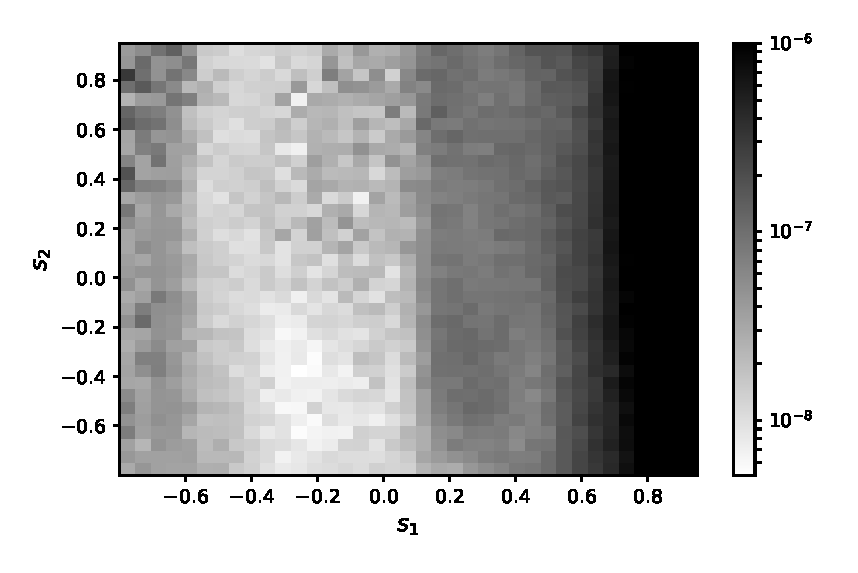
\includegraphics[width=\linewidth]{mse_countour_spins}
		\end{minipage}
    \end{minipage}\hfill
    \begin{minipage}{\linewidth}
        \centering
	 	\begin{minipage}{\minipagesize\linewidth}
		    \centering
		    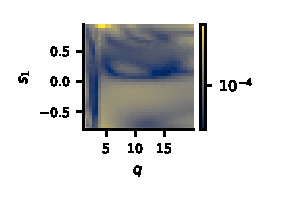
\includegraphics[width=\linewidth]{F_countour_q_s1}
		\end{minipage}\hfill
		\begin{minipage}{\minipagesize\linewidth}
		    \centering
		    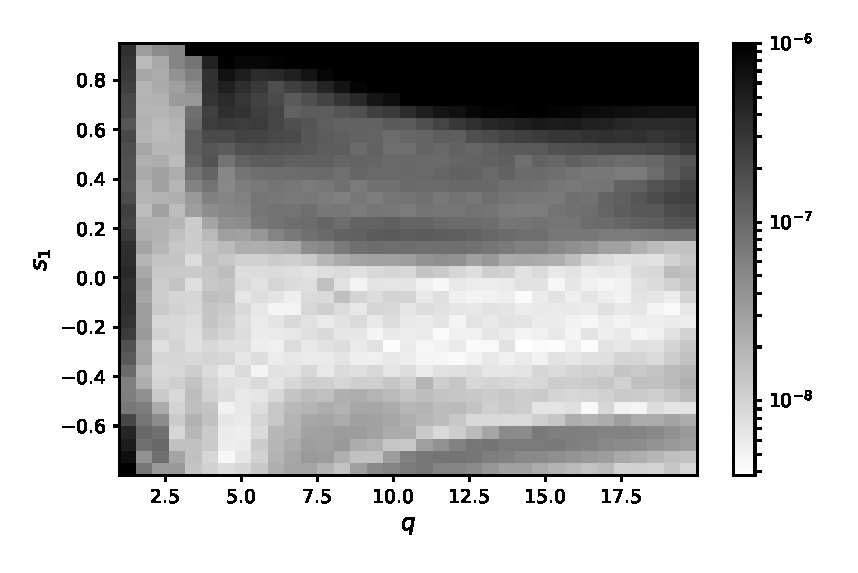
\includegraphics[width=\linewidth]{mse_countour_q_s1}
		\end{minipage}
    \end{minipage}
	\caption{We report test mismatch and mse for the first PC of the phase, as a function of the orbital parameters $\vartheta = (q, M, s_1, s_2)$. The histograms holds $145061$ waveforms, with randomly drawn parameters.
In the left column, the color mesh refers to test mismatch; in the right column, we report test mse on the first PC.
On the x-y we display values of two physical quantities, each discretized in $35$ bins.
On top row, we display $q$ vs $M$ dependence. On central row, we present spins dependence $s_1$ vs $s_2$. On bottom row, we show $q$ vs $s_1$ dependence.
Each wave starts $\SI{8}{s}$ before merger.
\sschmidt{Do we keep mse column???}
}
	\label{fig:countour}
\end{figure}
%\clearpage
}
%%%
\par
By looking at the top line of \ref{fig:countour}, we note that the mse does not depend on $M$. This was to be expected because the total mass dependence is inserted analytically within the model.
We note also that both $\mathcal{F}$ and mse depend (quite strongly) on $q$.
\par
In the center line of \ref{fig:countour}, we displayed the dependence on spins.
As long as the $s_1$ dependence is considered, the most striking feature is the inverse correlation of mismatch and mse for the first phase PC.
This means that, being non-leading, spin contribution are not important for the first PC but become dominant at higher order of PCs.
Indeed, the values of the first PC are well correlated with mismatch in the case of $q$. See~\cite{Ohme2013PCA_GW} for a closely related discussion on PCA components and its dependence on physical parameter.
\sschmidt{Is it fine to cite this? Is it relevant?}
\par
Apart from this feature, we note that the mismatch tends to grow for low values of $s_1$: the fit is less reliable in such regions.
\BS{[why it is not symmetric in the spins? are they treated
    differently? Based on the WF morphology/variation I would expect:
    (i) for up-down spins accuracy similar to nospin, and (ii) for down-down a higher
    accuracy than up-up ... but maybe this is naive...]}
\par
In the third row of \ref{fig:countour}, we displayed the dependence on $q$ and $s_1$, the variables on which the error depends more.
We note again the inverse correlation between the mismatch and mse, when considering the $s_1$ dependence.
%%%%%%%%%%%%%%%%%%
%%%%%%%%%%%%%%%
\subsection{Runtime analysis} \label{sec:runtime}
We now asses the time performances of our model.
We are interested to make a comparison with both \texttt{TEOBResumS}
(the train model) and \texttt{SEOBNRv4\_ROM} \cite{}.
%
\paragraph{Comparison with \texttt{TEOBResumS}}
When dealing with a real detection scenario, we are often interested in generating a WF which starts from a given frequency $f_{min}$, which is usually set by the detector's sensitivity window. Thus, it is crucial to measure the speed up that our model can provide in performing such task.
We define the speed up $\mathcal{S}$ as the ratio between the runtime of benchmark model and the runtime of \texttt{mlgw} to produce the a waveform starting from a given $f_{min}$. Each waveform is produced with constant total mass $M = 100 M_{\odot}$ and random parameters; the WF is sampled at $f_{sam} = \SI{2048}{Hz}$.
We consider the two cases with $f_{min} = \SI{5}{Hz}$ and $f_{min} = \SI{20}{Hz}$; the first choice refers to the hypotetical lower bound for the sentivity of the Einstein telescope (ET), while the second is close to that of Advanced-LIGO/Virgo.
In figure~\ref{fig:time_performance_hist} we report the histogram of the measured speed up values for model \texttt{TEOBResumS}.
\BS{[Have you tried to plot the speedup result as a function of the
    parameter space, e.g. (q,s1+s2)? e.g. in a 2D scatter plot. Might help indicating which
    waveform a slower/faster and identifying the original of the two
    peaks (say, particolarly large q or values of spins)]}
  
\newcommand{\factor}{.9}
\begin{figure}
	\centering
	\begin{minipage}{\factor\linewidth}
	    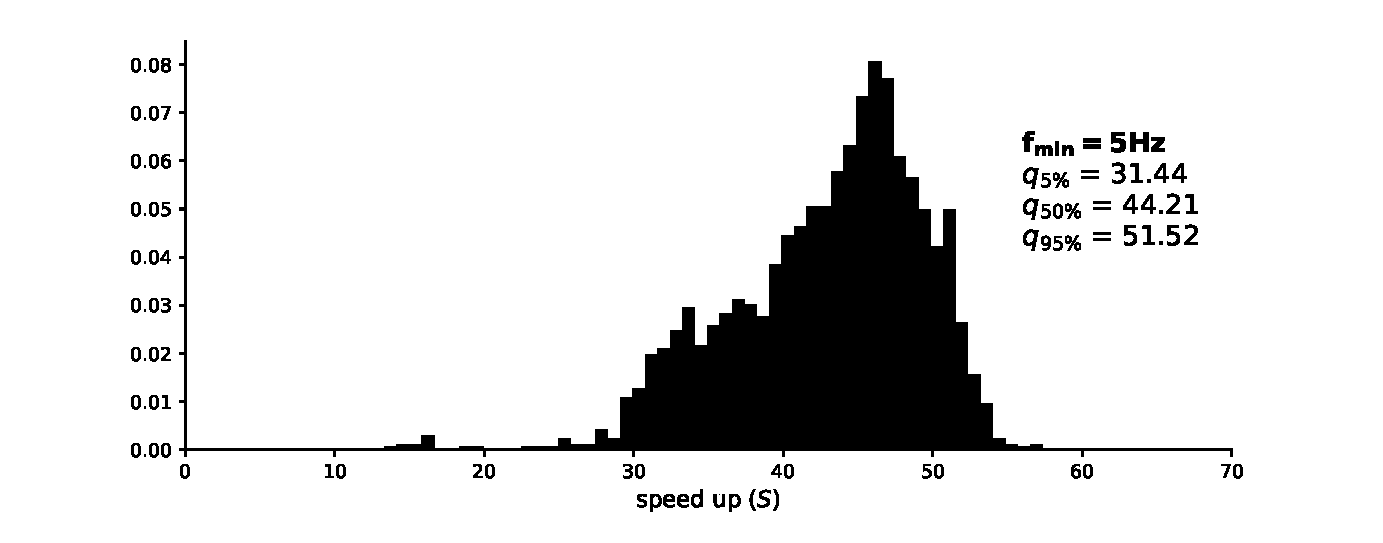
\includegraphics[width=\linewidth]{time_performance_hist_5}
	\end{minipage}\hfill
	\begin{minipage}{\factor\linewidth}
	    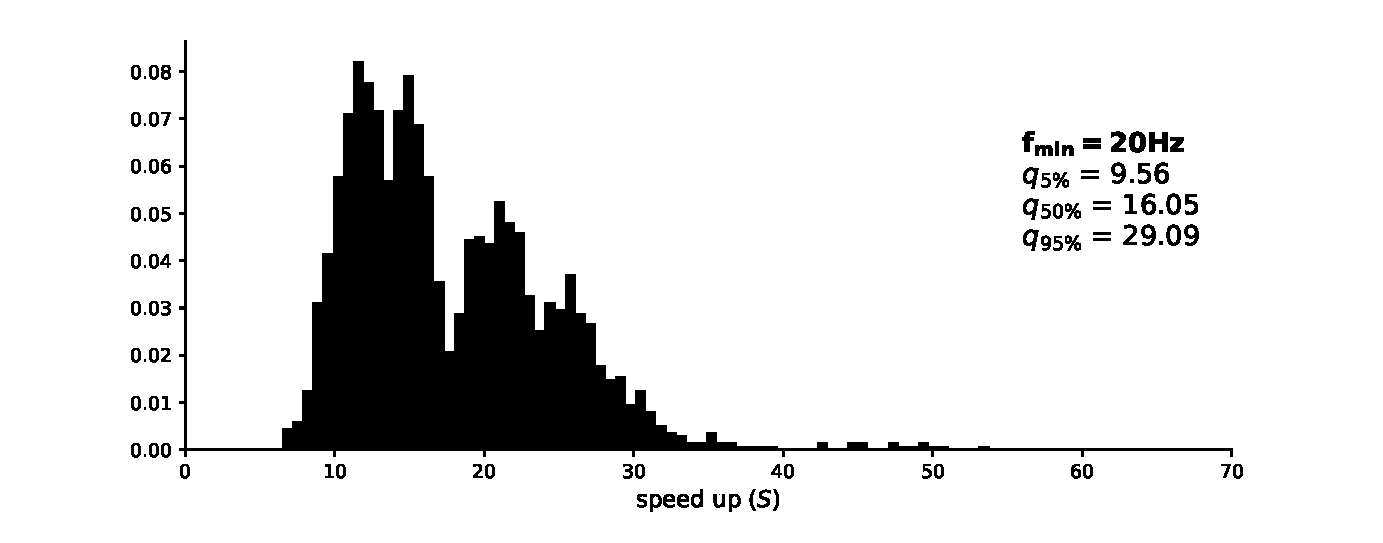
\includegraphics[width=\linewidth]{time_performance_hist_20}
	\end{minipage}

	\caption{
Histogram for values of the speed up given by \texttt{mlgw}, as compared with \texttt{TEOBResumS} model, computed on $N=2000$ test waveforms. Each WF is generated with random physical parameters and has a minimum frequency of $\SI{5}{Hz}$ (top panel) and $\SI{20}{Hz}$ (bottom panel).
We set a constant total mass $M=\SI{100}{M_\odot}$ and the sampling rate $f_{sam} = \SI{2048}{Hz}$.
We report the median value $q_{50\%}$ as well as the positions $q_{5\%}$ and $q_{95\%}$ of the 5th and 95th percentile.
\sschmidt{Are you really sure that two peaks are fine?? Understand this...}
}
	\label{fig:time_performance_hist}
\end{figure}
%%%%%%%%%%
\begin{figure}
	\centering
	\begin{minipage}{\factor\linewidth}
	    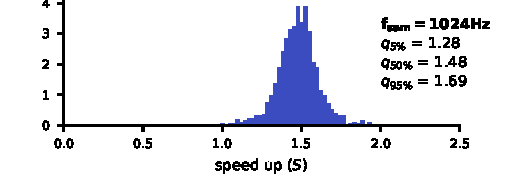
\includegraphics[width=\linewidth]{time_performance_hist_ROM_20_1024}
	\end{minipage}\hfill
	\begin{minipage}{\factor\linewidth}
	    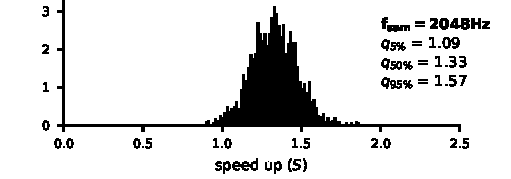
\includegraphics[width=\linewidth]{time_performance_hist_ROM_20_2048}
	\end{minipage}

	\caption{
Histograms for values of the speed up given by \texttt{mlgw}, as compared with ROM model \texttt{SEOBNRv4\_ROM}, computed on $N=2000$ test waveforms.
Each WF is generated with random physical parameters and has a sampling frequency $f_{sam}$ of $\SI{1024}{Hz}$ (top panel) and $\SI{2048}{Hz}$ (bottom panel).
We set a constant total mass $M=\SI{100}{M_\odot}$ and the same starting frequency $f_{min} = \SI{20}{Hz}$.
We report the median value $q_{50\%}$ as well as the positions $q_{5\%}$ and $q_{95\%}$ of the 5th and 95th percentile.
}
	\label{fig:time_performance_hist_ROM}
\end{figure}

%%%%%%%%%%
We see that in both cases a substantial speed up is achieved. The speed up is higher for longer WFs
\footnote{This is clearly understood: a longer WF requires more computation for a EOB model, while roughly the same amount of work is done by \texttt{mlgw}}, 
making our model particulary convenient for advanced detectors, with a larger sensitivity window.
\par
\paragraph{Comparison with \texttt{SEOBNRv4\_ROM}}
In figure~\ref{fig:time_performance_hist_ROM} we report the histogram of the measured speed up values for model \texttt{SEOBNRv4\_ROM}, which is now the state of the art for the WF generation time.
The comparison is made as above only for $f_{min} = \SI{20}{Hz}$; the ROM has not been built for $f_{min} = \SI{5}{Hz}$.
As the ROM model yields WFs in frequency domain, in the time comparison we included a fast Fourier trasform (FFT) of the time domain WF of \texttt{mlgw}. This is to ensure that we evaluate the two model at the same conditions.
Interestingly, the time taken by the FFT (in the \texttt{numpy}
implementation) is similar to that required to generate a WF. Thus for
a WF in FD, our model cannot be substantially faster, due to the
limitation imposed by the FFT.\BS{[How about the interpolation to the
    uniform grid required before the FFT?]}
\sschmidt{I don't get the point here...}
\par
We note the the performances are quite similar to each other.
If a lower sampling rate is employed, \texttt{mlgw} slighly improves its performances.
\par
It is important to stress that \texttt{mlgw} is written in pure
Python, while \texttt{SEOBNRv4\_ROM} is coded in C.
In fact, a python code could be easily accelerated (i.e. parellelized, run on GPUs, etc...) with dedicated libraries, thus allowing to push the code performance further.
%
\sschmidt{Is it ok now??}
%
Furthermore, \texttt{mlgw} is more efficient in reconstructing the
waveforms: it requires only $O(5\cdot 10^3)$ WFs for the training,
while in order to build a ROM as many as $O(5\cdot 10^5)$ WFs are
required. 
\par
%%%
\paragraph{Profiling}
It is interesting to have a knowledge of the time spent by \texttt{mlgw} in each stage of the WF generation procedure.
We generate $100$ waves with random physical parameters and we measure the CPU time spent to execute each basic task.
In table \ref{tab:profiling}, we compare the results for two values of $N_{grid}$.
\begin{table}
	\def\arraystretch{1.5}
	\begin{tabular}{ l c c }
		\multirow{2}{*}{Task (for 100 WFs)}& \multicolumn{2}{c}{CPU time (ms)}\\
			&$N_{grid} = 10^3$	& $N_{grid} = 10^5$\\
	\hline \hline
		 Generation of raw WF 			& $6.9 \; (46.9\%)$	& $7 \; (1.6\%)$ \\ 
	\hline
		 Interpolation to the user grid & $4.5 \; (30.6\%)$	& $194 \; (45.3\%)$ \\ 
	\hline
		 Post processing 				& $1.7 \; (11.6\%)$	& $206 \; (48.1\%)$ \\
	\hline
		 Total							& $14.7 \; (100\%)$ &  $428 \; (100.0\%)$ \\
	\hline \hline
	\end{tabular}
	\caption{
Time taken by different stages of the generation of $100$ waveforms; data refers to two different values of $N_{grid}$.
Generation of raw WF refers to the computation of the strain $h_{FIT}$ as produced by a ML model. Interpolation to user grid evaluates the WF on the grid chosen by the user. In the post-processing phase, the dependence on $d_L$, $\iota$ and $\varphi_0$ is included.
}
	\label{tab:profiling}
\end{table}
\par
We see that the cost of generating the raw WF does not depend on the number of grid points. On the other hand, the interpolation and the post processing depends on $N_{grid}$ and their cost grows dramatically as the user requires more and more points.
It is important to stress that the latter two tasks are slow only because they deal with a large amount of points. Indeed they perform trivial and ``quick" operations and their execution relies on well optimized \texttt{numpy} routines.
If such an amount of datapoints is required, very little space is left for speed up.
\par

\section{Application to GWTC-1}
\label{sec:GWTC1}

We test the implementation of our MLGW-TEOBResumS model on the public data from GWTC-1, the first GW catalog~\cite{}.
We trained \texttt{mlgw} in the range $\mathcal{P} = [1,20]\times[-0.8,0.95]\times[-0.8,0.95]$ and we set $\tau_{min} = \SI{4}{s/M_\odot}$.
The GWTC-1 catalog consists of 10 BBH systems and a BNS system. Because of the training of the WF model, we do not analyse GW170817, the BNS system, and concentrate exclusively on the BBH signals. Our parameter estimation algorithm is \texttt{gwmodel}~\cite{} a publicly available infrastructure 
written in a mixture of \texttt{Python} and \texttt{cython} that serves as interface for the parallel nested sampling implementation \texttt{cpnest}~\cite{}. 
The analysis of each BBH system is set up as follows; we choose a total of 2000 Live Points, four parallel MCMC chains with a maximum length of 5000 steps to ensure that each successive sample is independent of the previous. These settings yield an average of $\sim$ 15000 posterior samples and 
evidence calculations that are accurate to the first decimal digit. For each BBH system we choose prior distributions as described in the GWTC-1 release paper~\cite{}. Finally, and critically, to ensure that our results can be compared fairly to published ones, we employ the power spectral densities released as part of GWTC-1. No calibration uncertainty model is assumed for these runs. 
\begin{figure*}[]
	\centering
    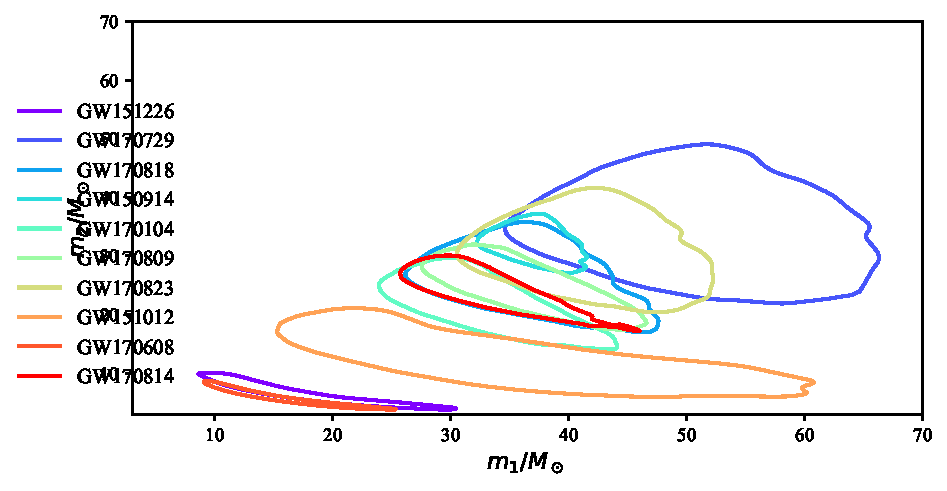
\includegraphics[width=.75\linewidth]{img/posterior_masses_source.pdf}
	\caption{
Two-dimensional posterior distributions for the component masses for all BBH systems in GWTC-1. The contours enclose the 90\% credible regions.
The figure shall be compared with figure 10 in \cite{Abbott_2019_GWTC} (left panel).
}
	\label{fig:summary-masses}
\end{figure*}

\begin{figure*}[]
	\centering
    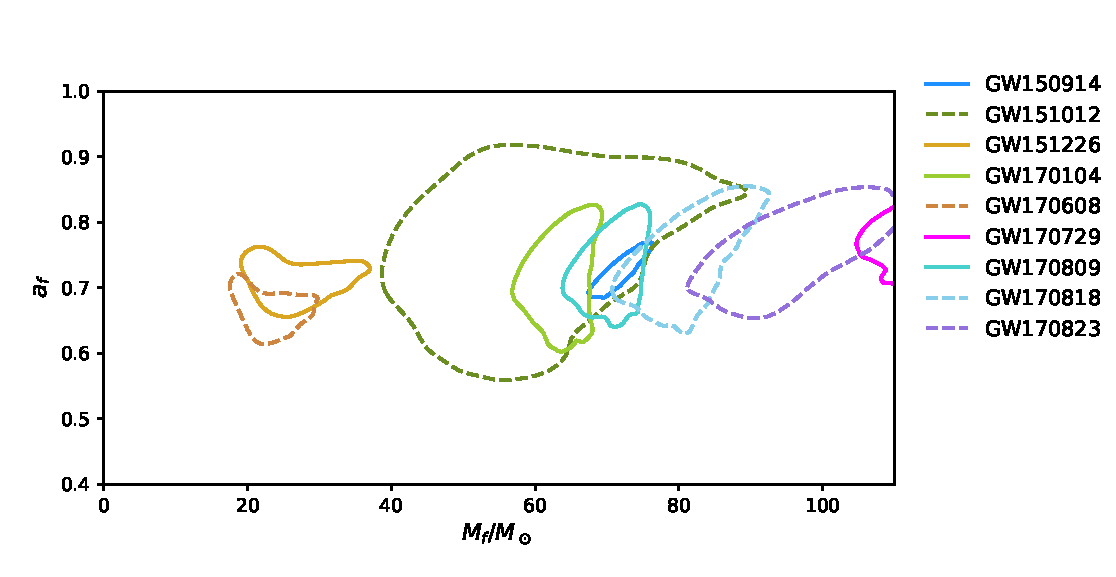
\includegraphics[width=.75\linewidth]{img/final_spin_mass.pdf}
	\caption{
Two-dimensional posterior distributions for the final masses and spins for all BBH systems in GWTC-1. The contours enclose the 90\% credible regions.
The figure shall be compared with figure 10 in \cite{Abbott_2019_GWTC} (right panel).
}
	\label{fig:summary-final-state}
\end{figure*}

Figure~\ref{fig:summary-masses}~\ref{fig:summary-final-state} and Table~\ref{tab:summary} summarise our results. In Table~\ref{tab:summary} we report exclusively 
summary statistic for the intrinsic parameters of the system. All mass parameters quoted are in the source frame. The redshift of each BBH is estimated 
from its luminosity distance posterior and converted into a redshift by assuming the cosmological parameters given in Ref.~\cite{}.

\begin{table*}[]
\centering
\caption{Summary table for the inferred intrinsic parameters from MLGW and the released GWTC-1 credible intervals. All mass parameters quoted are computed in the source frame, see the text for details of the calculation. For GWTC-1 we report results from Table III, thus coming from averaging over two waveform models. The uncertainties correspond to the 90\% credible intervals.
\sschmidt{What about $q$ in GWTC-1?? Is not in GWTC-1 paper...}
}
\label{tab:summary}
\begin{tabular}{cccccc|ccccc}
                              & \multicolumn{5}{c}{MLGW}                                                   & \multicolumn{5}{c|}{GWTC-1}                                                \\ \hline
\multicolumn{1}{c|}{Event}    & $m_1/M_\odot$ & $m_2/M_\odot$ & $\mathcal{M}/M_\odot$ & $q$ & $\chi_{eff}$ & $m_1/M_\odot$ & $m_2/M_\odot$ & $\mathcal{M}/M_\odot$ & $q$ & $\chi_{eff}$ \\ \hline
\multicolumn{1}{c|}{GW150914} & $36.36_{-2.64}^{+4.72}$& $32.64_{-4.44}^{+2.93}$& $29.87_{-1.50}^{+1.95}$& $0.91_{-0.21}^{+0.08}$& $0.14_{-0.10}^{+0.10}$&    $35.6_{-3.1}^{+4.7}$           &   $30.6_{-4.4}^{+3.0}$            & $28.6_{-1.5}^{+1.7}$                      & ?? & $-0.01_{-0.13}^{+0.12}$              \\
\multicolumn{1}{c|}{GW151012}& $34.51_{-14.46}^{+21.37}$& $11.67_{-4.46}^{+6.92}$& $16.86_{-2.68}^{+3.01}$& $0.33_{-0.19}^{+0.56}$& $0.53_{-0.33}^{+0.20}$&   $23.2_{-5.5}^{+14.9}$            &   $13.6_{-4.8}^{+4.1}$            &  $15.2_{-1.2}^{+2.1}$                     & ?? & $0.05_{-0.2}^{+0.32}$              \\
\multicolumn{1}{c|}{GW151226} & $16.44_{-5.52}^{+12.15}$& $6.38_{-2.18}^{+2.86}$& $8.72_{-0.27}^{+0.45}$& $0.39_{-0.24}^{+0.45}$& $0.32_{-0.14}^{+0.24}$&   $13.7_{-3.2}^{+8.8}$            & $7.7_{-2.5}^{+2.2}$               &  $8.9_{-0.3}^{+0.3}$                     & ?? & $0.18_{-0.12}^{+0.20}$              \\
\multicolumn{1}{c|}{GW170104} & $31.16_{-4.77}^{+10.55}$& $22.69_{-6.91}^{+4.70}$& $22.83_{-2.06}^{+2.64}$& $0.74_{-0.35}^{+0.23}$& $0.23_{-0.15}^{+0.15}$&  $30.8_{-5.6}^{+7.3}$             & $20.0_{-4.6}^{+4.9}$              & $21.4_{-1.8}^{2.2}$                       & ?? & $-0.04_{-0.21}^{+0.17}$             \\
\multicolumn{1}{c|}{GW170608} & $15.45_{-5.05}^{+7.60}$& $5.61_{-1.50}^{+2.32}$& $7.90_{-0.17}^{+0.25}$& $0.36_{-0.18}^{+0.40}$& $0.25_{-0.17}^{+0.20}$&  $11.0_{-1.7}^{+5.5}$             & $7.6_{-2.2}^{+1.4}$              &      $7.9_{-0.2}^{+0.2}$                  & ?? &   $0.03_{-0.07}^{+0.19}$           \\
\multicolumn{1}{c|}{GW170729} & $50.04_{-9.98}^{+13.97}$& $34.78_{-9.73}^{+9.78}$& $35.73_{-5.08}^{+7.08}$& $0.71_{-0.28}^{+0.26}$& $0.51_{-0.23}^{+0.18}$&  $50.2_{-10.2}^{+16.2}$             &  $34.0_{-10.0}^{+9.1}$             & $35.4_{-4.8}^{6.5}$                      & ?? & $0.37_{-0.25}^{+0.21}$              \\
\multicolumn{1}{c|}{GW170809} & $35.35_{-5.43}^{+8.88}$& $25.17_{-5.91}^{+4.81}$& $25.69_{-1.74}^{+2.35}$& $0.72_{-0.27}^{+0.25}$& $0.24_{-0.14}^{+0.16}$&    $35.0_{-5.9}^{+8.3}$           &                 $23.8_{-5.2}^{+5.1}$                     &  $24.9_{-1.7}^{+2.1}$   & & $0.08_{-0.17}^{+0.17}$             \\
\multicolumn{1}{c|}{GW170814}& $31.35_{-3.48}^{+10.70}$& $25.24_{-6.40}^{+3.16}$& $24.40_{-1.29}^{+1.50}$& $0.81_{-0.36}^{+0.17}$& $0.19_{-0.11}^{+0.12}$&  $30.6_{-3.0}^{+5.6}$             &               $25.2_{-4.0}^{+2.8}$&   $24.1_{-1.1}^{+1.4}$                    & ?? &   $0.06_{-0.12}^{+0.12}$           \\
\multicolumn{1}{c|}{GW170818} &$34.62_{-5.18}^{+11.61}$& $27.09_{-7.80}^{+5.59}$& $26.34_{-2.77}^{+4.03}$& $0.80_{-0.37}^{+0.18}$& $0.28_{-0.19}^{+0.20}$&   $35.4_{-4.7}^{+7.5}$            &               $26.7_{-5.2}^{+4.3}$& $26.5_{-1.7}^{+2.1}$                      & ?? &  $-0.09_{-0.21}^{+0.18}$            \\
\multicolumn{1}{c|}{GW170823} & $40.69_{-6.68}^{+10.21}$& $31.17_{-8.09}^{+7.13}$& $30.63_{-3.75}^{+5.01}$& $0.78_{-0.30}^{+0.19}$& $0.31_{-0.20}^{+0.18}$&  $39.5_{-6.7}^{+11.2}$             &               $29.0_{-7.8}^{+6.7}$&   $29.2_{-3.6}^{+4.6}$                    & ?? &   $0.09_{-0.26}^{+0.22}$           \\ \hline
\end{tabular}
\end{table*}

Our results are, in general, extremely similar to what published by the LVK Collaboration. This is reassuring as it validates both the WF model hereby presented as well as the data analysis scheme and sampler implemented\footnote{However, a full validation of the algorithm is presented in ~\cite{}.}.
We do note certain interesting aspects that are worth mention; for instance, MLGW tends to recover slightly larger chirp masses and slightly 
smaller mass ratios compared to GWTC-1. At the same  time, the value of $\chi_{eff}$ also tends to be slightly larger. These differences are, in general, negligible, but nevertheless indicative of the differences in the physics input in the approximant. The results in Table~\ref{tab:summary} have been produced using the TEOBResumS MLGW model. TEOBResumS has a treatment of the angular momenta coupling that is quite different from SEOBNRv4 and hence from the IMRPhenom family of waveforms that, albeit indirectly, is calibrated on SEOBNR. As mentioned, the differences are, at least at the signal-to-noises in GWTC-1, very small, but we find very interesting that a different spin coupling prescription has the potential to impact the inferred spin posteriors, prime example is GW170729, and thus the mass parameters. 
In light of our findings, we think that the resolution of the spin physics is paramount for an accurate and free from systematics inference of astrophysical properties such as the BBH mass and spin distributions.

%%%%%%%%%%%%%%%%%%%
\section{Final remarks and future prospects}
\label{sec:end}

\BS{[I think this needs a bit more structure. All the material is there it is matter of re-organinzing shortening] e.g. logic following from the paper could be
\begin{itemize}
\item Short summary of the key ML ingredients of the method and how to go beyond /improve those
\item Short summary of the WF performances and how to improve them, extension of mlgw to modes, precession, and freq-domain, NR data etc
\item Short summary of PE application and future prospects
\end{itemize}
}

We built a ready-to-use Machine Learning model which generates the (dominant quadrupole) time-domain gravitational wave signal from a binary Black Hole coalescence in the non precessing case. The code is released as the package \texttt{mlgw}, publicly available at
\href{https://pypi.org/project/mlgw/}{pypi.org/project/mlgw/}. The user might install it with the command \texttt{pip install mlgw}.
The model consists of a PCA model to reduce the dimensionality of the 22 mode (decomposed in amplitude and phase). A regression (a MoE model) is performed to infer a relation from the orbital paramters to the low dimensional representation of the WF.
\par
It is important to stress that our model is very simple, i.e. it has a very little number of trainable paramters and it is not expensive to train, and flexible, i.e. it works for a large range of paramters and for long waveforms.
In \cite{Chua_2019}, a ML model for GW generation is built, with similar performances. However, the reduced dimension space is considerably larger ($O(200)$) than ours ($O(10)$).
In \cite{khan2020gravitationalwave}, the low dimensional space has a similar dimension $O(30)$ and the ML model achieves a similar performance in the time execution (when computed on a CPU). They manage to achieve a better accuracy $O(2\cdot10^{-5})$ but they generate significantly shorter WFs ($f_{min} = \SI{15}{Hz}$ for $M = \SI{60}{M_{\odot}}$ against $f_{min} \simeq \SI{2.5}{Hz}$) and employ a larger training time ($O(\SI{6}{hours})$ against $O(\SI{6}{minutes})$).
\par
Remarkably, we discovered that a PCA is able to reproduce a high dimensional wave using a few number of variables.
On the other hand, the MoE model is currently it is the ``bottleneck" of the model accuracy. For this reason, we explored several alternative regression methods, including neural networks, but none of them showed dramaticaly better performance: perhaps much more computational power and a larger training set are required to improve the fit performances any better.
\par
Despite this, our model shows excellent agreement with the underlying training set. At test time, the median mismatch is $\bar{\mathcal{F}}\sim 5 \cdot 10^{-4}$.
Furthermore, a single WF generations takes $\SI{0.1}{}-\SI{5}{ms}$ (depending mostly on the number of grid points required by the user), which is a factor of $\sim 40$ faster than the underlying train model.
\texttt{mlgw} slightly outperforms a ROM, which is currently the state-of-the-art for quick generation.
\par
Our ML framework allows for several generalization, which might build a more accurate WF generator.
First of all, it is quite straightforward to include higher order modes (HMs) in the WF computation. Different regressions, each for each mode, might be done as we already did for the 22 mode. A future update of \texttt{mlgw} is in program.
Second, also the precession effects might be included in the model.
The precession dynamics could be inserted as a single spin parameter $s_P$ \cite{Schmidt2015Precession} and the WF depencence on $s_P$ can be fitted together with the other orbital parameters.
\par
Furthermore, our model could be trained on the publicly available NR waveforms 
catalogs (see e.g.~\cite{Mroue:2013xna,Boyle:2019kee,Healy:2019jyf} and it would provide the best generalization of 
the numerical waveform, dispensing with the EOB models altogether.
Unfortunately, at the moment there are too few NR waveforms ($O(10^2)$) available to perform a reliable 
training\footnote{At least $O(5\cdot 10^3)$ waveforms are required.}
and the improvement shall wait until enough NR waveforms are available.
Moreover, NR waveforms are too short to be used as they are and probably, an extension (e.g. by hybridization with EOB waveforms)
towards the early inspiral is needed to compute any kind of NR-based surrogate model.
\par
Latly, we expect our ML approach to work for every kind of source for which a training set of 
waveforms is available. Machine learning models to generate WFs might be crucial in 
the future, where signals from a number of different sources are expected to be detected. In that scenario, 
a parameter estimation must be able to detect among different source and this will require a lot 
of computational work. Speed up will be more pressing.
\par

Our work opens up interesting opportunities in GW data analysis (seaches and parameter estimation), both because of its speed and of the closed form expression for the WF.

Due to its speed, \texttt{mlgw} could be employed for a systematic comparison between different waveform models, directly on data.
By training (and the training procedure is also quick) \texttt{mlgw} with different waveform models, it will be possible to compare their predictions on several observed events. This could allow to detect systematic biases or to prefer a model over another by means of Bayesian model selection (i.e. by comparing different model evidences).
We started this program by analysing GWTC-1 with \texttt{mlgw} trained on \texttt{TEOBResumS} and highlited some differences in the predictions as compared to the published results (see section \ref{sec:GWTC1}). Future work might repeat such an analysis on other models or with more observations.
\par
Furthermore, as shown in fig.~\ref{fig:time_performance_hist}, the model is most useful whenever a long waveform is required: in such case, the speed-up gets even more substantial.
This is crucial for the detection of low frequency signals, as is the case for ET. The analysis of such signals can be performed in the same time required to deal with shorter signals: it will become feasible, even with a small amount of resourches, \textit{without any loss of WF quality}.
%In \cite{} (\sschmidt{plot in email}), it was shown that training model TEOBResumS matches accurately the numerical relativity WFs, even in the case of ET noise curve is used (see plot in the email). Since our model closely reproduces TEOBResumS, it is likely to achieve the target accuracy for the employment in the ET data analysis.
%\sschmidt{Here I wanted to include the plot sent by Nagar. Is it in a paper? Do we include it here? Or do we just skip it??}
\par
A closed form expression for the gradients of the waveform with respect to the orbital parameters $m_1,m_2, {s}_1,{s}_2$
\footnote{The computation of gradient is already included in the \texttt{mlgw} package.}
could give an advantage on the parameter estimation procedure by using the Hamiltonian MonteCarlo (HM).
HM \cite{betancourt2017hamiltonianMC}~\cite{Porter2014Hamiltonian_MonteCarlo} is a variant of Markov chain Montecarlo, which employs gradients of the likelihood (which depends on the gradient of the waveform) to perform an effective sampling of the posterior distibution. The sampling chain conveges faster to the steady state by ``find quickly" the high density regions, thus offering a speed up of the PE.
\par
Another option, so far never explored, is to use the gradients of the WF for a fast exploration of the likelihood landscape. With any gradient based optimizer, it should be easy to jump to a \textit{local} maximum of the likelihood. Such information might be helpful to reliably locate a \textit{global} maximum of the likelihood.
The ability to quickly locate a global maximum could speed up the searches and the parameter estimation.
\par
\sschmidt{Frase a effetto finale??}



%%%%%%%%%%%%%%%%%%%%%%%%%%%%%%%
%%% OLD
%%%%%%%%%%%%%%%%%%%%%%%%%%%%%%%
%We built a ready-to-use Machine Learning model which generates the (dominant quadrupole) gravitational wave signal from a binary Black Hole coalescence in the non precessing case. The code is released as the package \texttt{mlgw} available via the \texttt{PyPI} Python package repository.
%Our model shows excellent agreement with the underlying training set. At test times the median mismatch is $\bar{\mathcal{F}}\sim 5 \cdot 10^{-4}$. Lastly, the generation time from \texttt{mlgw} is smaller than the underlying training model by a factor of $\sim 40$, for a waveform starting at a frequency of $\SI{5}{Hz}$.
%\texttt{mlgw} performance matches closely those of a ROM, which is currently the state-of-the-art for a quick generation.
%Moreover, it was successfully employed for the analysis of the GWTC-1 catalog of waveforms.
%\par
%Remarkably, we discovered that a PCA is able to reproduce a high dimensional wave using a few number of variables. As for the regression model itself, the MoE model, currently it is the ``bottleneck" of the model accuracy. For this reason, we explored several alternative regression methods, including neural networks, but none of them showed dramaticaly better performance.
%Note that underfitting may be an issue whenever the training model shows intrinsic noise due to mis-modeling, e.g. relations that are supposed to be continuous are not, or even due to poor numerical integration schemes.
%\par
%Our work opens up interesting opportunities in GW data analysis.
%As shown in fig.~\ref{fig:time_performance_hist}, the model is the most useful whenever a long waveform is required. Furthermore, the waveform generation time does not depend on the complexity of the underlying surrogate model. The training WFs can be computed with high accuracy, also at high computational cost, without affecting the performance of the WF generation.
%\par
%This fact is crucial for detection of low frequency signals, as is the case for ET. The analysis of such signals can be performed in the same time required to deal with shorter signals: it will become feasible, even with a small amount of resourches, \textit{without any loss of WF quality}.
%In \cite{} (\sschmidt{plot in email}), it was shown that training model TEOBResumS matches accurately the numerical relativity WFs, even in the case of ET noise curve is used (see plot in the email). Since our model closely reproduces TEOBResumS, it is likely to achieve the target accuracy for the employment in the ET data analysis.
%\sschmidt{Here I wanted to include the plot sent by Nagar. Is it in a paper? Do we include it here? Or do we just skip it??}
%\par


%The fact that a parameter estimation with \texttt{mlgw} is remarkably fast opens up the opportunity for a systematic comparison between different waveform model.
%By training (and the training procedure is moderately quick) \texttt{mlgw} with different waveform models, it will be possible to compare their predictions on several observed events. This could allow to detect systematic biases or to prefer a model over another by means of Bayesian model selection (i.e. by comparing different model evidences).
%We started this program by analysing GWTC-1 with \texttt{mlgw} trained on \texttt{TEOBResumS} and highlited some differences in the predictions as compared to the published results (see section \ref{sec:GWTC1}). Future work might repeat such an analysis on other models or with more observations.
%\par
%However, our work is far from being over and several issues still require attention.
%\par
%First of all, it is quite straightforward to include higher order modes (HMs) in the WF computation. Different regressions, each for each mode, might be done as we already did for the 22 mode. This is the most natural generalization of our work and a future update of \texttt{mlgw} is in program.
%\par
%Second, the potential speed up of parameter estimation can be even higher, if we take advantage of the closed form expression of the waveform provided by our model.
%Indeed, a closed form expression for the WF allows for prompt computation of the gradients with respect to the orbital parameters $ \boldsymbol{\vartheta} = (m_1,m_2, {s}_1,{s}_2) $.
%Hamiltonian Montecarlo \cite{betancourt2017hamiltonianMC}~\cite{Porter2014Hamiltonian_MonteCarlo}, a variant of Markov chain Montecarlo, employs gradients of the waveform to perform an effective sampling of the posterior distibution, which is able to ``find quickly" the high density regions.
%Porter and Carré \cite{Porter2014Hamiltonian_MonteCarlo} applied Hamiltonian Montecarlo to parameter estimation. However, they only use analytical waveforms, which completely neglects the late inspiral and the merger.
%Our Machine Learning model could, in principle, extend the application of Hamiltonian Montecarlo to waveform which included also late inspiral, merger and ringdown.
%It would provide a state-of-the-art accurate parameter estimation and, at the same time, it will offer a substantial speed up.
%We believe that this is a promising option and it is among the natural continuations of our work.
%\par
%Another option, so far never explored, is to use the gradients of the WF for a fast exploration of the likelihood landscape. With any gradient based optimizer, it should be easy to jump to a \textit{local} maximum of the likelihood. Such information might be helpful to reliably locate a \textit{global} maximum of the likelihood. Once a global maximum is found, the sampling from the posterior distribution should be quicker to perform, yielding an improvement to the overall analysis.
%\par
%In our model we did not consider precessing system. We made this choice to keep the problem simple.
%The expertise gained for the simple non precessing case can be applied to deal with the complicacies posed by the precessing case.
%A good starting point is given in \cite{Schmidt2015Precession}, where the whole spin dynamics (dependent on 6 parameters) is mapped to a simpler problem, where the precession is controlled by a single parameter $s_P$.
%The waveform dependence on the effective spin parameter $s_P$ can be fitted by a ML model in the same fashion of the other orbital parameters, thus avoid to complicate (much) the regression problem.

%All EOB models provides numerical solutions to approximate form of the Einstein equations. They are useful to catch 
%the dominant physics but we expect them to show a degree of inaccuracy, especially close to coalescence.
%Numerical relativity solves numerically Einstein equations without approximations and so far yields the physically most 
%complete available solutions. However, NR waveforms by themselves cannot be used in parameter estimation because
%of their sparse coverage of the parameter space. Our model could be trained on the publicly available NR waveforms 
%catalogs (see e.g.~\cite{Mroue:2013xna,Boyle:2019kee,Healy:2019jyf} and it would provide the best generalization of 
%the numerical waveform. If the model proved to be reliable and effective,  we could dispense with the EOB models 
%altogether and use only NR inputs for a parameter estimation.  This would ensure that all the relevant physics close 
%to merger is adequately captured. 
%Unfortunately, at the moment there are too few NR waveforms ($O(10^2)$) available to perform a reliable 
%training: we need at least $O(10^3)$ waveforms. However, in the future we expect more and more waveforms 
%to be included in the dataset, eventually allowing for a reliable training. Furthermore, currently available 
%NR waveforms are too short to be used as they are, and an extension (e.g. by hybridization with EOB waveforms)
%towards the early inspiral is needed to compute any kind of NR-based surrogate model.

%Our machine learning approach to signal generation is very flexible and provides a general framework 
%for a ML-based WF generator. We expect it to work for every source for which a number of training 
%waveforms are available. Machine learning models for various wealth of sources might be crucial in 
%the future, where signals from a number of different sources are expected to be detected. In that scenario, 
%a parameter estimation must be able to detect among different source and this will require a lot 
%of computational work. Speed up will be more pressing.

%A Python implementation of the model is released in the package \texttt{mlgw}, publicly available at \href{https://pypi.org/project/mlgw/}{pypi.org/project/mlgw/}. The user might install it with the command \texttt{pip install mlgw}. The package provides also the gradients $\frac{\partial h}{\partial\vartheta_i}$ of the waveform, computed analytically from equation \ref{eq:model}.



